\documentclass[1p]{elsarticle_modified}
%\bibliographystyle{elsarticle-num}

%\usepackage[colorlinks]{hyperref}
%\usepackage{abbrmath_seonhwa} %\Abb, \Ascr, \Acal ,\Abf, \Afrak
\usepackage{amsfonts}
\usepackage{amssymb}
\usepackage{amsmath}
\usepackage{amsthm}
\usepackage{scalefnt}
\usepackage{amsbsy}
\usepackage{kotex}
\usepackage{caption}
\usepackage{subfig}
\usepackage{color}
\usepackage{graphicx}
\usepackage{xcolor} %% white, black, red, green, blue, cyan, magenta, yellow
\usepackage{float}
\usepackage{setspace}
\usepackage{hyperref}

\usepackage{tikz}
\usetikzlibrary{arrows}

\usepackage{multirow}
\usepackage{array} % fixed length table
\usepackage{hhline}

%%%%%%%%%%%%%%%%%%%%%
\makeatletter
\renewcommand*\env@matrix[1][\arraystretch]{%
	\edef\arraystretch{#1}%
	\hskip -\arraycolsep
	\let\@ifnextchar\new@ifnextchar
	\array{*\c@MaxMatrixCols c}}
\makeatother %https://tex.stackexchange.com/questions/14071/how-can-i-increase-the-line-spacing-in-a-matrix
%%%%%%%%%%%%%%%

\usepackage[normalem]{ulem}

\newcommand{\msout}[1]{\ifmmode\text{\sout{\ensuremath{#1}}}\else\sout{#1}\fi}
%SOURCE: \msout is \stkout macro in https://tex.stackexchange.com/questions/20609/strikeout-in-math-mode

\newcommand{\cancel}[1]{
	\ifmmode
	{\color{red}\msout{#1}}
	\else
	{\color{red}\sout{#1}}
	\fi
}

\newcommand{\add}[1]{
	{\color{blue}\uwave{#1}}
}

\newcommand{\replace}[2]{
	\ifmmode
	{\color{red}\msout{#1}}{\color{blue}\uwave{#2}}
	\else
	{\color{red}\sout{#1}}{\color{blue}\uwave{#2}}
	\fi
}

\newcommand{\Sol}{\mathcal{S}} %segment
\newcommand{\D}{D} %diagram
\newcommand{\A}{\mathcal{A}} %arc


%%%%%%%%%%%%%%%%%%%%%%%%%%%%%5 test

\def\sl{\operatorname{\textup{SL}}(2,\Cbb)}
\def\psl{\operatorname{\textup{PSL}}(2,\Cbb)}
\def\quan{\mkern 1mu \triangleright \mkern 1mu}

\theoremstyle{definition}
\newtheorem{thm}{Theorem}[section]
\newtheorem{prop}[thm]{Proposition}
\newtheorem{lem}[thm]{Lemma}
\newtheorem{ques}[thm]{Question}
\newtheorem{cor}[thm]{Corollary}
\newtheorem{defn}[thm]{Definition}
\newtheorem{exam}[thm]{Example}
\newtheorem{rmk}[thm]{Remark}
\newtheorem{alg}[thm]{Algorithm}

\newcommand{\I}{\sqrt{-1}}
\begin{document}

%\begin{frontmatter}
%
%\title{Boundary parabolic representations of knots up to 8 crossings}
%
%%% Group authors per affiliation:
%\author{Yunhi Cho} 
%\address{Department of Mathematics, University of Seoul, Seoul, Korea}
%\ead{yhcho@uos.ac.kr}
%
%
%\author{Seonhwa Kim} %\fnref{s_kim}}
%\address{Center for Geometry and Physics, Institute for Basic Science, Pohang, 37673, Korea}
%\ead{ryeona17@ibs.re.kr}
%
%\author{Hyuk Kim}
%\address{Department of Mathematical Sciences, Seoul National University, Seoul 08826, Korea}
%\ead{hyukkim@snu.ac.kr}
%
%\author{Seokbeom Yoon}
%\address{Department of Mathematical Sciences, Seoul National University, Seoul, 08826,  Korea}
%\ead{sbyoon15@snu.ac.kr}
%
%\begin{abstract}
%We find all boundary parabolic representation of knots up to 8 crossings.
%
%\end{abstract}
%\begin{keyword}
%    \MSC[2010] 57M25 
%\end{keyword}
%
%\end{frontmatter}

%\linenumbers
%\tableofcontents
%
\newcommand\colored[1]{\textcolor{white}{\rule[-0.35ex]{0.8em}{1.4ex}}\kern-0.8em\color{red} #1}%
%\newcommand\colored[1]{\textcolor{white}{ #1}\kern-2.17ex	\textcolor{white}{ #1}\kern-1.81ex	\textcolor{white}{ #1}\kern-2.15ex\color{red}#1	}

{\Large $\underline{12a_{0510}~(K12a_{0510})}$}

\setlength{\tabcolsep}{10pt}
\renewcommand{\arraystretch}{1.6}
\vspace{1cm}\begin{tabular}{m{100pt}>{\centering\arraybackslash}m{274pt}}
\multirow{5}{120pt}{
	\centering
	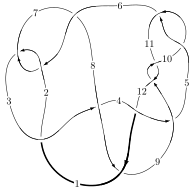
\includegraphics[width=112pt]{../../../GIT/diagram.site/Diagrams/png/1311_12a_0510.png}\\
\ \ \ A knot diagram\footnotemark}&
\allowdisplaybreaks
\textbf{Linearized knot diagam} \\
\cline{2-2}
 &
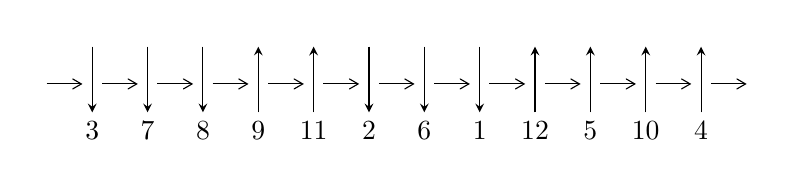
\begin{tikzpicture}[x=20pt, y=17pt]
	% nodes
	\node (C0) at (0, 0) {};
	\node (C1) at (1, 0) {};
	\node (C1U) at (1, +1) {};
	\node (C1D) at (1, -1) {3};

	\node (C2) at (2, 0) {};
	\node (C2U) at (2, +1) {};
	\node (C2D) at (2, -1) {7};

	\node (C3) at (3, 0) {};
	\node (C3U) at (3, +1) {};
	\node (C3D) at (3, -1) {8};

	\node (C4) at (4, 0) {};
	\node (C4U) at (4, +1) {};
	\node (C4D) at (4, -1) {9};

	\node (C5) at (5, 0) {};
	\node (C5U) at (5, +1) {};
	\node (C5D) at (5, -1) {11};

	\node (C6) at (6, 0) {};
	\node (C6U) at (6, +1) {};
	\node (C6D) at (6, -1) {2};

	\node (C7) at (7, 0) {};
	\node (C7U) at (7, +1) {};
	\node (C7D) at (7, -1) {6};

	\node (C8) at (8, 0) {};
	\node (C8U) at (8, +1) {};
	\node (C8D) at (8, -1) {1};

	\node (C9) at (9, 0) {};
	\node (C9U) at (9, +1) {};
	\node (C9D) at (9, -1) {12};

	\node (C10) at (10, 0) {};
	\node (C10U) at (10, +1) {};
	\node (C10D) at (10, -1) {5};

	\node (C11) at (11, 0) {};
	\node (C11U) at (11, +1) {};
	\node (C11D) at (11, -1) {10};

	\node (C12) at (12, 0) {};
	\node (C12U) at (12, +1) {};
	\node (C12D) at (12, -1) {4};
	\node (C13) at (13, 0) {};

	% arrows
	\draw[->,>={angle 60}]
	(C0) edge (C1) (C1) edge (C2) (C2) edge (C3) (C3) edge (C4) (C4) edge (C5) (C5) edge (C6) (C6) edge (C7) (C7) edge (C8) (C8) edge (C9) (C9) edge (C10) (C10) edge (C11) (C11) edge (C12) (C12) edge (C13) ;	\draw[->,>=stealth]
	(C1U) edge (C1D) (C2U) edge (C2D) (C3U) edge (C3D) (C4D) edge (C4U) (C5D) edge (C5U) (C6U) edge (C6D) (C7U) edge (C7D) (C8U) edge (C8D) (C9D) edge (C9U) (C10D) edge (C10U) (C11D) edge (C11U) (C12D) edge (C12U) ;
	\end{tikzpicture} \\
\hhline{~~} \\& 
\textbf{Solving Sequence} \\ \cline{2-2} 
 &
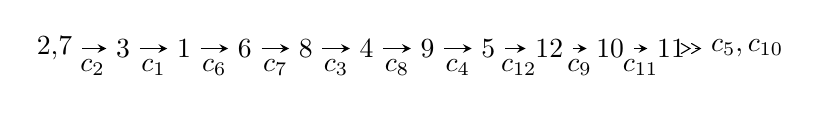
\begin{tikzpicture}[x=22pt, y=7pt]
	% node
	\node (A0) at (-1/8, 0) {2,7};
	\node (A1) at (1, 0) {3};
	\node (A2) at (2, 0) {1};
	\node (A3) at (3, 0) {6};
	\node (A4) at (4, 0) {8};
	\node (A5) at (5, 0) {4};
	\node (A6) at (6, 0) {9};
	\node (A7) at (7, 0) {5};
	\node (A8) at (8, 0) {12};
	\node (A9) at (9, 0) {10};
	\node (A10) at (10, 0) {11};
	\node (C1) at (1/2, -1) {$c_{2}$};
	\node (C2) at (3/2, -1) {$c_{1}$};
	\node (C3) at (5/2, -1) {$c_{6}$};
	\node (C4) at (7/2, -1) {$c_{7}$};
	\node (C5) at (9/2, -1) {$c_{3}$};
	\node (C6) at (11/2, -1) {$c_{8}$};
	\node (C7) at (13/2, -1) {$c_{4}$};
	\node (C8) at (15/2, -1) {$c_{12}$};
	\node (C9) at (17/2, -1) {$c_{9}$};
	\node (C10) at (19/2, -1) {$c_{11}$};
	\node (A11) at (45/4, 0) {$c_{5},c_{10}$};

	% edge
	\draw[->,>=stealth]	
	(A0) edge (A1) (A1) edge (A2) (A2) edge (A3) (A3) edge (A4) (A4) edge (A5) (A5) edge (A6) (A6) edge (A7) (A7) edge (A8) (A8) edge (A9) (A9) edge (A10) ;
	\draw[->>,>={angle 60}]	
	(A10) edge (A11);
\end{tikzpicture} \\ 

\end{tabular} \\

\footnotetext{
The image of knot diagram is generated by the software ``\textbf{Draw programme}" developed by Andrew Bartholomew(\url{http://www.layer8.co.uk/maths/draw/index.htm\#Running-draw}), where we modified some parts for our purpose(\url{https://github.com/CATsTAILs/LinksPainter}).
}\phantom \\ \newline 
\centering \textbf{Ideals for irreducible components\footnotemark of $X_{\text{par}}$} 
 
\begin{align*}
I^u_{1}&=\langle 
u^{96}- u^{95}+\cdots-2 u+1\rangle \\
\\
\end{align*}
\raggedright * 1 irreducible components of $\dim_{\mathbb{C}}=0$, with total 96 representations.\\
\footnotetext{All coefficients of polynomials are rational numbers. But the coefficients are sometimes approximated in decimal forms when there is not enough margin.}
\newpage
\renewcommand{\arraystretch}{1}
\centering \section*{I. $I^u_{1}= \langle u^{96}- u^{95}+\cdots-2 u+1 \rangle$}
\flushleft \textbf{(i) Arc colorings}\\
\begin{tabular}{m{7pt} m{180pt} m{7pt} m{180pt} }
\flushright $a_{2}=$&$\begin{pmatrix}1\\0\end{pmatrix}$ \\
\flushright $a_{7}=$&$\begin{pmatrix}0\\u\end{pmatrix}$ \\
\flushright $a_{3}=$&$\begin{pmatrix}1\\u^2\end{pmatrix}$ \\
\flushright $a_{1}=$&$\begin{pmatrix}- u^2+1\\- u^4\end{pmatrix}$ \\
\flushright $a_{6}=$&$\begin{pmatrix}u\\u\end{pmatrix}$ \\
\flushright $a_{8}=$&$\begin{pmatrix}- u^3\\- u^3+u\end{pmatrix}$ \\
\flushright $a_{4}=$&$\begin{pmatrix}- u^8+u^6- u^4+1\\- u^8+2 u^6-2 u^4+2 u^2\end{pmatrix}$ \\
\flushright $a_{9}=$&$\begin{pmatrix}- u^9+2 u^7-3 u^5+2 u^3- u\\- u^{11}+u^9-2 u^7+u^5- u^3+u\end{pmatrix}$ \\
\flushright $a_{5}=$&$\begin{pmatrix}u^{28}-5 u^{26}+\cdots+u^2+1\\u^{30}-4 u^{28}+\cdots-2 u^4+u^2\end{pmatrix}$ \\
\flushright $a_{12}=$&$\begin{pmatrix}u^{20}-3 u^{18}+7 u^{16}-10 u^{14}+10 u^{12}-7 u^{10}+u^8+2 u^6-3 u^4+u^2+1\\u^{20}-4 u^{18}+10 u^{16}-18 u^{14}+23 u^{12}-24 u^{10}+18 u^8-10 u^6+3 u^4\end{pmatrix}$ \\
\flushright $a_{10}=$&$\begin{pmatrix}- u^{51}+8 u^{49}+\cdots-6 u^5+3 u^3\\- u^{51}+9 u^{49}+\cdots- u^3+u\end{pmatrix}$ \\
\flushright $a_{11}=$&$\begin{pmatrix}u^{82}-13 u^{80}+\cdots+u^2+1\\u^{82}-14 u^{80}+\cdots+2 u^4+u^2\end{pmatrix}$\\&\end{tabular}
\flushleft \textbf{(ii) Obstruction class $= -1$}\\~\\
\flushleft \textbf{(iii) Cusp Shapes $= 4 u^{94}-60 u^{92}+\cdots-4 u^3+6$}\\~\\
\newpage\renewcommand{\arraystretch}{1}
\flushleft \textbf{(iv) u-Polynomials at the component}\newline \\
\begin{tabular}{m{50pt}|m{274pt}}
Crossings & \hspace{64pt}u-Polynomials at each crossing \\
\hline $$\begin{aligned}c_{1},c_{7}\end{aligned}$$&$\begin{aligned}
&u^{96}+31 u^{95}+\cdots-4 u^2+1
\end{aligned}$\\
\hline $$\begin{aligned}c_{2},c_{6}\end{aligned}$$&$\begin{aligned}
&u^{96}- u^{95}+\cdots-2 u+1
\end{aligned}$\\
\hline $$\begin{aligned}c_{3}\end{aligned}$$&$\begin{aligned}
&u^{96}+u^{95}+\cdots-16 u+1
\end{aligned}$\\
\hline $$\begin{aligned}c_{4}\end{aligned}$$&$\begin{aligned}
&u^{96}- u^{95}+\cdots+16 u+1
\end{aligned}$\\
\hline $$\begin{aligned}c_{5},c_{10}\end{aligned}$$&$\begin{aligned}
&u^{96}+u^{95}+\cdots+2 u+1
\end{aligned}$\\
\hline $$\begin{aligned}c_{8}\end{aligned}$$&$\begin{aligned}
&u^{96}-7 u^{95}+\cdots-71328 u+6545
\end{aligned}$\\
\hline $$\begin{aligned}c_{9},c_{11}\end{aligned}$$&$\begin{aligned}
&u^{96}-31 u^{95}+\cdots-4 u^2+1
\end{aligned}$\\
\hline $$\begin{aligned}c_{12}\end{aligned}$$&$\begin{aligned}
&u^{96}+7 u^{95}+\cdots+71328 u+6545
\end{aligned}$\\
\hline
\end{tabular}\\~\\
\newpage\renewcommand{\arraystretch}{1}
\flushleft \textbf{(v) Riley Polynomials at the component}\newline \\
\begin{tabular}{m{50pt}|m{274pt}}
Crossings & \hspace{64pt}Riley Polynomials at each crossing \\
\hline $$\begin{aligned}c_{1},c_{7},c_{9}\\c_{11}\end{aligned}$$&$\begin{aligned}
&y^{96}+69 y^{95}+\cdots-8 y+1
\end{aligned}$\\
\hline $$\begin{aligned}c_{2},c_{5},c_{6}\\c_{10}\end{aligned}$$&$\begin{aligned}
&y^{96}-31 y^{95}+\cdots-4 y^2+1
\end{aligned}$\\
\hline $$\begin{aligned}c_{3},c_{4}\end{aligned}$$&$\begin{aligned}
&y^{96}-3 y^{95}+\cdots+32 y+1
\end{aligned}$\\
\hline $$\begin{aligned}c_{8},c_{12}\end{aligned}$$&$\begin{aligned}
&y^{96}+25 y^{95}+\cdots+1210281936 y+42837025
\end{aligned}$\\
\hline
\end{tabular}\\~\\
\newpage\flushleft \textbf{(vi) Complex Volumes and Cusp Shapes}
$$\begin{array}{c|c|c}  
\text{Solutions to }I^u_{1}& \I (\text{vol} + \sqrt{-1}CS) & \text{Cusp shape}\\
 \hline 
\begin{aligned}
u &= \phantom{-}0.668621 + 0.743484 I\end{aligned}
 & -1.66618 - 3.03949 I & \phantom{-0.000000 } 0 \\ \hline\begin{aligned}
u &= \phantom{-}0.668621 - 0.743484 I\end{aligned}
 & -1.66618 + 3.03949 I & \phantom{-0.000000 } 0 \\ \hline\begin{aligned}
u &= -0.671467 + 0.758961 I\end{aligned}
 & -2.04180 - 2.66465 I & \phantom{-0.000000 } 0 \\ \hline\begin{aligned}
u &= -0.671467 - 0.758961 I\end{aligned}
 & -2.04180 + 2.66465 I & \phantom{-0.000000 } 0 \\ \hline\begin{aligned}
u &= \phantom{-}0.838636 + 0.518053 I\end{aligned}
 & \phantom{-}1.78716 + 0.07371 I & \phantom{-0.000000 } 0 \\ \hline\begin{aligned}
u &= \phantom{-}0.838636 - 0.518053 I\end{aligned}
 & \phantom{-}1.78716 - 0.07371 I & \phantom{-0.000000 } 0 \\ \hline\begin{aligned}
u &= \phantom{-}1.022380 + 0.120604 I\end{aligned}
 & -3.68776 - 3.29743 I & \phantom{-0.000000 } 0 \\ \hline\begin{aligned}
u &= \phantom{-}1.022380 - 0.120604 I\end{aligned}
 & -3.68776 + 3.29743 I & \phantom{-0.000000 } 0 \\ \hline\begin{aligned}
u &= -0.956778 + 0.147180 I\end{aligned}
 & -1.78716 + 0.07371 I & \phantom{-0.000000 } 0 \\ \hline\begin{aligned}
u &= -0.956778 - 0.147180 I\end{aligned}
 & -1.78716 - 0.07371 I & \phantom{-0.000000 } 0 \\ \hline\begin{aligned}
u &= -1.029200 + 0.147717 I\end{aligned}
 & \phantom{-0.000000 -}5.56148 I & \phantom{-0.000000 } 0 \\ \hline\begin{aligned}
u &= -1.029200 - 0.147717 I\end{aligned}
 & \phantom{-0.000000 } -5.56148 I & \phantom{-0.000000 } 0 \\ \hline\begin{aligned}
u &= -1.042110 + 0.066897 I\end{aligned}
 & -7.33598 - 3.27045 I & \phantom{-0.000000 } 0 \\ \hline\begin{aligned}
u &= -1.042110 - 0.066897 I\end{aligned}
 & -7.33598 + 3.27045 I & \phantom{-0.000000 } 0 \\ \hline\begin{aligned}
u &= \phantom{-}1.042500 + 0.077924 I\end{aligned}
 & -7.84437 - 2.48794 I & \phantom{-0.000000 } 0 \\ \hline\begin{aligned}
u &= \phantom{-}1.042500 - 0.077924 I\end{aligned}
 & -7.84437 + 2.48794 I & \phantom{-0.000000 } 0 \\ \hline\begin{aligned}
u &= \phantom{-}0.928290 + 0.486480 I\end{aligned}
 & -3.57263 + 5.11647 I & \phantom{-0.000000 } 0 \\ \hline\begin{aligned}
u &= \phantom{-}0.928290 - 0.486480 I\end{aligned}
 & -3.57263 - 5.11647 I & \phantom{-0.000000 } 0 \\ \hline\begin{aligned}
u &= -0.929772 + 0.502774 I\end{aligned}
 & -4.38563 + 0.62113 I & \phantom{-0.000000 } 0 \\ \hline\begin{aligned}
u &= -0.929772 - 0.502774 I\end{aligned}
 & -4.38563 - 0.62113 I & \phantom{-0.000000 } 0 \\ \hline\begin{aligned}
u &= -0.700212 + 0.794099 I\end{aligned}
 & \phantom{-}2.47685 - 3.08229 I & \phantom{-0.000000 } 0 \\ \hline\begin{aligned}
u &= -0.700212 - 0.794099 I\end{aligned}
 & \phantom{-}2.47685 + 3.08229 I & \phantom{-0.000000 } 0 \\ \hline\begin{aligned}
u &= \phantom{-}1.050030 + 0.136772 I\end{aligned}
 & -6.42062 - 5.30599 I & \phantom{-0.000000 } 0 \\ \hline\begin{aligned}
u &= \phantom{-}1.050030 - 0.136772 I\end{aligned}
 & -6.42062 + 5.30599 I & \phantom{-0.000000 } 0 \\ \hline\begin{aligned}
u &= -1.051930 + 0.143074 I\end{aligned}
 & -5.49564 + 11.08280 I & \phantom{-0.000000 } 0 \\ \hline\begin{aligned}
u &= -1.051930 - 0.143074 I\end{aligned}
 & -5.49564 - 11.08280 I & \phantom{-0.000000 } 0 \\ \hline\begin{aligned}
u &= -0.687870 + 0.811992 I\end{aligned}
 & \phantom{-0.000000 } -5.27036 I & \phantom{-0.000000 } 0 \\ \hline\begin{aligned}
u &= -0.687870 - 0.811992 I\end{aligned}
 & \phantom{-0.000000 -}5.27036 I & \phantom{-0.000000 } 0 \\ \hline\begin{aligned}
u &= -0.930368 + 0.072614 I\end{aligned}
 & -1.83592 + 0.18281 I & \phantom{-0.000000 } 0 \\ \hline\begin{aligned}
u &= -0.930368 - 0.072614 I\end{aligned}
 & -1.83592 - 0.18281 I & \phantom{-0.000000 } 0\\
 \hline 
 \end{array}$$\newpage$$\begin{array}{c|c|c}  
\text{Solutions to }I^u_{1}& \I (\text{vol} + \sqrt{-1}CS) & \text{Cusp shape}\\
 \hline 
\begin{aligned}
u &= \phantom{-}0.689278 + 0.816429 I\end{aligned}
 & \phantom{-}0.98870 + 11.03430 I & \phantom{-0.000000 } 0 \\ \hline\begin{aligned}
u &= \phantom{-}0.689278 - 0.816429 I\end{aligned}
 & \phantom{-}0.98870 - 11.03430 I & \phantom{-0.000000 } 0 \\ \hline\begin{aligned}
u &= \phantom{-}0.702443 + 0.810718 I\end{aligned}
 & \phantom{-}6.42062 + 5.30599 I & \phantom{-0.000000 } 0 \\ \hline\begin{aligned}
u &= \phantom{-}0.702443 - 0.810718 I\end{aligned}
 & \phantom{-}6.42062 - 5.30599 I & \phantom{-0.000000 } 0 \\ \hline\begin{aligned}
u &= -0.912613 + 0.567303 I\end{aligned}
 & -1.31450 + 2.17183 I & \phantom{-0.000000 } 0 \\ \hline\begin{aligned}
u &= -0.912613 - 0.567303 I\end{aligned}
 & -1.31450 - 2.17183 I & \phantom{-0.000000 } 0 \\ \hline\begin{aligned}
u &= \phantom{-}0.724039 + 0.796746 I\end{aligned}
 & \phantom{-}4.38563 - 0.62113 I & \phantom{-0.000000 } 0 \\ \hline\begin{aligned}
u &= \phantom{-}0.724039 - 0.796746 I\end{aligned}
 & \phantom{-}4.38563 + 0.62113 I & \phantom{-0.000000 } 0 \\ \hline\begin{aligned}
u &= \phantom{-}0.895137 + 0.209877 I\end{aligned}
 & -1.29372 - 4.71443 I & \phantom{-0.000000 -}0. + 7.32005 I \\ \hline\begin{aligned}
u &= \phantom{-}0.895137 - 0.209877 I\end{aligned}
 & -1.29372 + 4.71443 I & \phantom{-0.000000 } 0. - 7.32005 I \\ \hline\begin{aligned}
u &= \phantom{-}0.762641 + 0.766889 I\end{aligned}
 & \phantom{-}3.60402 - 0.95351 I & \phantom{-0.000000 } 0 \\ \hline\begin{aligned}
u &= \phantom{-}0.762641 - 0.766889 I\end{aligned}
 & \phantom{-}3.60402 + 0.95351 I & \phantom{-0.000000 } 0 \\ \hline\begin{aligned}
u &= -0.757759 + 0.793359 I\end{aligned}
 & \phantom{-}4.92325 - 3.35595 I & \phantom{-0.000000 } 0 \\ \hline\begin{aligned}
u &= -0.757759 - 0.793359 I\end{aligned}
 & \phantom{-}4.92325 + 3.35595 I & \phantom{-0.000000 } 0 \\ \hline\begin{aligned}
u &= -0.784352 + 0.786872 I\end{aligned}
 & \phantom{-}7.84437 + 2.48794 I & \phantom{-0.000000 } 0 \\ \hline\begin{aligned}
u &= -0.784352 - 0.786872 I\end{aligned}
 & \phantom{-}7.84437 - 2.48794 I & \phantom{-0.000000 } 0 \\ \hline\begin{aligned}
u &= \phantom{-}0.805888 + 0.773211 I\end{aligned}
 & \phantom{-}2.04180 - 2.66465 I & \phantom{-0.000000 } 0 \\ \hline\begin{aligned}
u &= \phantom{-}0.805888 - 0.773211 I\end{aligned}
 & \phantom{-}2.04180 + 2.66465 I & \phantom{-0.000000 } 0 \\ \hline\begin{aligned}
u &= \phantom{-}0.931057 + 0.621319 I\end{aligned}
 & \phantom{-}1.29372 - 4.71443 I & \phantom{-0.000000 } 0 \\ \hline\begin{aligned}
u &= \phantom{-}0.931057 - 0.621319 I\end{aligned}
 & \phantom{-}1.29372 + 4.71443 I & \phantom{-0.000000 } 0 \\ \hline\begin{aligned}
u &= -0.806863 + 0.783033 I\end{aligned}
 & \phantom{-}3.03143 + 8.19865 I & \phantom{-0.000000 } 0 \\ \hline\begin{aligned}
u &= -0.806863 - 0.783033 I\end{aligned}
 & \phantom{-}3.03143 - 8.19865 I & \phantom{-0.000000 } 0 \\ \hline\begin{aligned}
u &= -0.965059 + 0.582350 I\end{aligned}
 & -4.92325 + 3.35595 I & \phantom{-0.000000 } 0 \\ \hline\begin{aligned}
u &= -0.965059 - 0.582350 I\end{aligned}
 & -4.92325 - 3.35595 I & \phantom{-0.000000 } 0 \\ \hline\begin{aligned}
u &= \phantom{-}0.970481 + 0.590990 I\end{aligned}
 & -4.27532 - 9.11947 I & \phantom{-0.000000 } 0 \\ \hline\begin{aligned}
u &= \phantom{-}0.970481 - 0.590990 I\end{aligned}
 & -4.27532 + 9.11947 I & \phantom{-0.000000 } 0 \\ \hline\begin{aligned}
u &= \phantom{-}0.927246 + 0.736499 I\end{aligned}
 & \phantom{-}1.66618 - 3.03949 I & \phantom{-0.000000 } 0 \\ \hline\begin{aligned}
u &= \phantom{-}0.927246 - 0.736499 I\end{aligned}
 & \phantom{-}1.66618 + 3.03949 I & \phantom{-0.000000 } 0 \\ \hline\begin{aligned}
u &= -0.930480 + 0.745778 I\end{aligned}
 & \phantom{-}2.64953 - 2.43631 I & \phantom{-0.000000 } 0 \\ \hline\begin{aligned}
u &= -0.930480 - 0.745778 I\end{aligned}
 & \phantom{-}2.64953 + 2.43631 I & \phantom{-0.000000 } 0\\
 \hline 
 \end{array}$$\newpage$$\begin{array}{c|c|c}  
\text{Solutions to }I^u_{1}& \I (\text{vol} + \sqrt{-1}CS) & \text{Cusp shape}\\
 \hline 
\begin{aligned}
u &= \phantom{-}0.960357 + 0.720758 I\end{aligned}
 & \phantom{-}2.99795 - 4.68596 I & \phantom{-0.000000 } 0 \\ \hline\begin{aligned}
u &= \phantom{-}0.960357 - 0.720758 I\end{aligned}
 & \phantom{-}2.99795 + 4.68596 I & \phantom{-0.000000 } 0 \\ \hline\begin{aligned}
u &= -0.949669 + 0.740584 I\end{aligned}
 & \phantom{-}7.33598 + 3.27045 I & \phantom{-0.000000 } 0 \\ \hline\begin{aligned}
u &= -0.949669 - 0.740584 I\end{aligned}
 & \phantom{-}7.33598 - 3.27045 I & \phantom{-0.000000 } 0 \\ \hline\begin{aligned}
u &= \phantom{-}1.000010 + 0.689675 I\end{aligned}
 & -2.64953 - 2.43631 I & \phantom{-0.000000 } 0 \\ \hline\begin{aligned}
u &= \phantom{-}1.000010 - 0.689675 I\end{aligned}
 & -2.64953 + 2.43631 I & \phantom{-0.000000 } 0 \\ \hline\begin{aligned}
u &= -0.969451 + 0.736227 I\end{aligned}
 & \phantom{-}4.27532 + 9.11947 I & \phantom{-0.000000 } 0 \\ \hline\begin{aligned}
u &= -0.969451 - 0.736227 I\end{aligned}
 & \phantom{-}4.27532 - 9.11947 I & \phantom{-0.000000 } 0 \\ \hline\begin{aligned}
u &= -1.003060 + 0.695382 I\end{aligned}
 & -3.03143 + 8.19865 I & \phantom{-0.000000 } 0 \\ \hline\begin{aligned}
u &= -1.003060 - 0.695382 I\end{aligned}
 & -3.03143 - 8.19865 I & \phantom{-0.000000 } 0 \\ \hline\begin{aligned}
u &= \phantom{-}0.990447 + 0.725417 I\end{aligned}
 & \phantom{-}3.57263 - 5.11647 I & \phantom{-0.000000 } 0 \\ \hline\begin{aligned}
u &= \phantom{-}0.990447 - 0.725417 I\end{aligned}
 & \phantom{-}3.57263 + 5.11647 I & \phantom{-0.000000 } 0 \\ \hline\begin{aligned}
u &= -1.001950 + 0.717439 I\end{aligned}
 & \phantom{-}1.56141 + 8.78593 I & \phantom{-0.000000 } 0 \\ \hline\begin{aligned}
u &= -1.001950 - 0.717439 I\end{aligned}
 & \phantom{-}1.56141 - 8.78593 I & \phantom{-0.000000 } 0 \\ \hline\begin{aligned}
u &= \phantom{-}1.006230 + 0.725835 I\end{aligned}
 & \phantom{-}5.49564 - 11.08280 I & \phantom{-0.000000 } 0 \\ \hline\begin{aligned}
u &= \phantom{-}1.006230 - 0.725835 I\end{aligned}
 & \phantom{-}5.49564 + 11.08280 I & \phantom{-0.000000 } 0 \\ \hline\begin{aligned}
u &= -1.013330 + 0.721341 I\end{aligned}
 & -0.98870 + 11.03430 I & \phantom{-0.000000 } 0 \\ \hline\begin{aligned}
u &= -1.013330 - 0.721341 I\end{aligned}
 & -0.98870 - 11.03430 I & \phantom{-0.000000 } 0 \\ \hline\begin{aligned}
u &= \phantom{-}1.014320 + 0.723773 I\end{aligned}
 & \phantom{-0.000000 } -16.8186 I & \phantom{-0.000000 } 0 \\ \hline\begin{aligned}
u &= \phantom{-}1.014320 - 0.723773 I\end{aligned}
 & \phantom{-0.000000 -}16.8186 I & \phantom{-0.000000 } 0 \\ \hline\begin{aligned}
u &= \phantom{-}0.620290 + 0.330583 I\end{aligned}
 & \phantom{-}1.83592 + 0.18281 I & \phantom{-}4.09090 + 0.35926 I \\ \hline\begin{aligned}
u &= \phantom{-}0.620290 - 0.330583 I\end{aligned}
 & \phantom{-}1.83592 - 0.18281 I & \phantom{-}4.09090 - 0.35926 I \\ \hline\begin{aligned}
u &= \phantom{-}0.403567 + 0.535727 I\end{aligned}
 & -2.99795 + 4.68596 I & -1.17578 - 2.89466 I \\ \hline\begin{aligned}
u &= \phantom{-}0.403567 - 0.535727 I\end{aligned}
 & -2.99795 - 4.68596 I & -1.17578 + 2.89466 I \\ \hline\begin{aligned}
u &= \phantom{-}0.178894 + 0.615558 I\end{aligned}
 & -1.56141 - 8.78593 I & \phantom{-}1.86370 + 7.76605 I \\ \hline\begin{aligned}
u &= \phantom{-}0.178894 - 0.615558 I\end{aligned}
 & -1.56141 + 8.78593 I & \phantom{-}1.86370 - 7.76605 I \\ \hline\begin{aligned}
u &= -0.361565 + 0.528636 I\end{aligned}
 & -3.60402 + 0.95351 I & -2.43173 - 2.83056 I \\ \hline\begin{aligned}
u &= -0.361565 - 0.528636 I\end{aligned}
 & -3.60402 - 0.95351 I & -2.43173 + 2.83056 I \\ \hline\begin{aligned}
u &= -0.189386 + 0.603096 I\end{aligned}
 & -2.47685 + 3.08229 I & \phantom{-}0.00392 - 2.94226 I \\ \hline\begin{aligned}
u &= -0.189386 - 0.603096 I\end{aligned}
 & -2.47685 - 3.08229 I & \phantom{-}0.00392 + 2.94226 I\\
 \hline 
 \end{array}$$\newpage$$\begin{array}{c|c|c}  
\text{Solutions to }I^u_{1}& \I (\text{vol} + \sqrt{-1}CS) & \text{Cusp shape}\\
 \hline 
\begin{aligned}
u &= \phantom{-}0.136116 + 0.585368 I\end{aligned}
 & \phantom{-}3.68776 - 3.29743 I & \phantom{-}8.17885 + 5.01878 I \\ \hline\begin{aligned}
u &= \phantom{-}0.136116 - 0.585368 I\end{aligned}
 & \phantom{-}3.68776 + 3.29743 I & \phantom{-}8.17885 - 5.01878 I \\ \hline\begin{aligned}
u &= \phantom{-}0.043930 + 0.554399 I\end{aligned}
 & \phantom{-}1.31450 + 2.17183 I & \phantom{-}6.03910 - 2.53826 I \\ \hline\begin{aligned}
u &= \phantom{-}0.043930 - 0.554399 I\end{aligned}
 & \phantom{-}1.31450 - 2.17183 I & \phantom{-}6.03910 + 2.53826 I \\ \hline\begin{aligned}
u &= -0.167581 + 0.505886 I\end{aligned}
 & \phantom{-0.000000 -}1.37910 I & \phantom{-0.000000 } 0. - 4.67220 I \\ \hline\begin{aligned}
u &= -0.167581 - 0.505886 I\end{aligned}
 & \phantom{-0.000000 } -1.37910 I & \phantom{-0.000000 -}0. + 4.67220 I\\
 \hline 
 \end{array}$$\newpage
\newpage\renewcommand{\arraystretch}{1}
\centering \section*{ II. u-Polynomials}
\begin{tabular}{m{50pt}|m{274pt}}
Crossings & \hspace{64pt}u-Polynomials at each crossing \\
\hline $$\begin{aligned}c_{1},c_{7}\end{aligned}$$&$\begin{aligned}
&u^{96}+31 u^{95}+\cdots-4 u^2+1
\end{aligned}$\\
\hline $$\begin{aligned}c_{2},c_{6}\end{aligned}$$&$\begin{aligned}
&u^{96}- u^{95}+\cdots-2 u+1
\end{aligned}$\\
\hline $$\begin{aligned}c_{3}\end{aligned}$$&$\begin{aligned}
&u^{96}+u^{95}+\cdots-16 u+1
\end{aligned}$\\
\hline $$\begin{aligned}c_{4}\end{aligned}$$&$\begin{aligned}
&u^{96}- u^{95}+\cdots+16 u+1
\end{aligned}$\\
\hline $$\begin{aligned}c_{5},c_{10}\end{aligned}$$&$\begin{aligned}
&u^{96}+u^{95}+\cdots+2 u+1
\end{aligned}$\\
\hline $$\begin{aligned}c_{8}\end{aligned}$$&$\begin{aligned}
&u^{96}-7 u^{95}+\cdots-71328 u+6545
\end{aligned}$\\
\hline $$\begin{aligned}c_{9},c_{11}\end{aligned}$$&$\begin{aligned}
&u^{96}-31 u^{95}+\cdots-4 u^2+1
\end{aligned}$\\
\hline $$\begin{aligned}c_{12}\end{aligned}$$&$\begin{aligned}
&u^{96}+7 u^{95}+\cdots+71328 u+6545
\end{aligned}$\\
\hline
\end{tabular}\newpage\renewcommand{\arraystretch}{1}
\centering \section*{ III. Riley Polynomials}
\begin{tabular}{m{50pt}|m{274pt}}
Crossings & \hspace{64pt}Riley Polynomials at each crossing \\
\hline $$\begin{aligned}c_{1},c_{7},c_{9}\\c_{11}\end{aligned}$$&$\begin{aligned}
&y^{96}+69 y^{95}+\cdots-8 y+1
\end{aligned}$\\
\hline $$\begin{aligned}c_{2},c_{5},c_{6}\\c_{10}\end{aligned}$$&$\begin{aligned}
&y^{96}-31 y^{95}+\cdots-4 y^2+1
\end{aligned}$\\
\hline $$\begin{aligned}c_{3},c_{4}\end{aligned}$$&$\begin{aligned}
&y^{96}-3 y^{95}+\cdots+32 y+1
\end{aligned}$\\
\hline $$\begin{aligned}c_{8},c_{12}\end{aligned}$$&$\begin{aligned}
&y^{96}+25 y^{95}+\cdots+1210281936 y+42837025
\end{aligned}$\\
\hline
\end{tabular}
\vskip 2pc
\end{document}